\documentclass[parskip=full,11pt]{scrartcl}
\usepackage[utf8]{inputenc}

\title{\Huge Parkview\\
    \LARGE \normalfont Performance Dashboard for Continuous Benchmarking of HPC Libraries}
\author{Chingun Ariunbat, Jamil Bagga, Walter Alexander B\"ottcher,\\Darius Schefer, Maximilian Schik}

% section numbers in margins:
\renewcommand\sectionlinesformat[4]{\makebox[0pt][r]{#3}#4}

% header & footer
\usepackage{scrlayer-scrpage}
%\lofoot{\today} % Date in footer
\refoot{\today}  % no idea what this does
\pagestyle{scrheadings}

\usepackage[sfdefault,light]{roboto}
\usepackage[T1]{fontenc}
\usepackage[english]{babel}
\usepackage[yyyymmdd]{datetime} % must be after babel
\usepackage{float}
\renewcommand{\dateseparator}{-}
\usepackage[colorlinks=true, linkcolor=blue]{hyperref}
\usepackage{amsmath} % for $\text{}$
\usepackage[nameinlink]{cleveref}
\crefname{figure}{Abb}{Abb}
\usepackage[section]{placeins}
\usepackage{xcolor}
\usepackage[nonumberlist, toc]{glossaries}     % provides glossary commands, [toc] to appear in table of contents
\usepackage{graphicx}
\usepackage{dirtree}
\graphicspath{ {./images/} }
\hypersetup{
	pdftitle={Design},
	bookmarks=true
}
\usepackage{QA}
\usepackage{csquotes} % provides \enquote{} command

\usepackage{booktabs}% http://ctan.org/pkg/booktabs
\newcommand{\tabitem}{~~\llap{\textbullet}~~}


\begin{document}

\maketitle
\begin{figure}[h]
	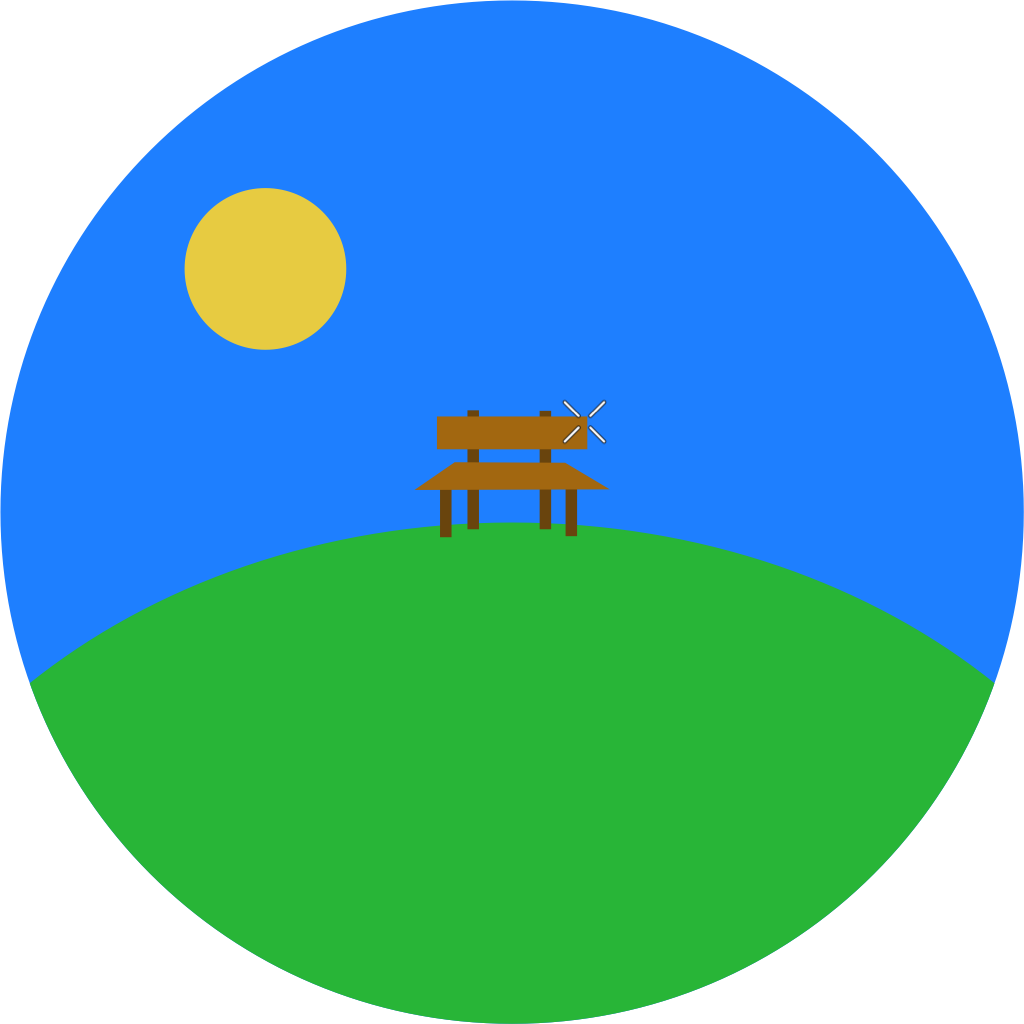
\includegraphics[width=11cm]{parkview.png}
	\centering
\end{figure}

\thispagestyle{empty}

\clearpage
\pagenumbering{arabic}

\tableofcontents
\clearpage

\section{Introduction}
This document describes in detail the quality assurance phase of \parkview{}, using automated unit tests for both the frontend and backend. This ensures that the implementation behaves according to the specification document.
\begin{itemize}
  \item The tests from the specification document are ran to check the functionality of the implementation
  \item Line and Branch coverage are given for relevant parts of the implementation
  \item A continuous integration pipeline is set up to check the functionality after changes are made.
\end{itemize}
\clearpage

\section{Scenarios}

\scenario{Inspecting Last Change}{scn:inspect_last_change}
{Ted: \Gls{user}, CI: \Gls{benchmarking system}}
{Ted works on a project that has \emph{PROJECT NAME} set up. He makes changes on a performance critical component. After that he pushes his changes to the repository. The CI sends its benchmark results to the system, which stores it in a persistent way. Ted opens the webapp and selects a benchmark. He sees a list of all recent changes. The changes without benchmark data are greyed out. Ted selects his newest change. He selects a device to take the benchmark data from. The change appears in a list of selected changes. Ted selects the \enquote{Create New Plot} option. A popup appears. Ted chooses the dimension he wants to inspect. After he configured his plot he decides to save the \gls{template} for later use. He selects the \enquote{Save Template} option. He enters a name for the \gls{template} and selects the \enquote{Save} option. After that he selects the \enquote{Generate Plot} option. Ted gets redirected to a new site where he can inspect his plot. He decides to send this plot to a coworker. He selects the \enquote{Share} option and a link gets displayed. He copies the link and sends it to his coworker.}

\scenario{Comparing Benchmarks}{scn:comp_benchmarks}
{Greta: \Gls{user}}
{Greta opens the webapp. She selects a benchmark. She selects two benchmarks by first picking a specific change and then a specific device. She opens the configuration popup by selecting the \enquote{Create New Plot} option. She wants to use a previously created \gls{template}. She selects the \enquote{Use Template} option and chooses her \gls{template} from a list of available ones. The settings specified in the \gls{template} get applied to the current \gls{configuration}. Greta makes final adjustments and then selects the \enquote{Generate Plot} option. After that she gets redirected to a new site where she can inspect her plot. Ted also wants to download the plot for use in his publication. He selects the \enquote{Export} option. He gets to choose between a seleciton of filetypes. He picks his preferred one. A link gets displayed leading to a download with the selected filetype.}

\scenario{Performance Tracking}{scn:perf_tracking}
{CI: \Gls{benchmarking system}}
{The CI runs a specific benchmark for a specific change on a specific device. It sends a POST request to the system containing the results and the benchmark type, change identification and device name. The system receives the results and stores them in a persistent database. It recognizes that the benchmark performance has dropped by a significant factor. The system triggers a hook that sends a message to the developer slack channel informing about the performance drop. It also publishes a comment under the change on GitHub.}


\clearpage

\appendix

%TBA

\end{document}
